\section{牛顿第二定律}\label{sec:03.02}

{\ziju{-0.01}牛顿第一定律确立了不受力情况下物体的运动性质。本节讨
论牛顿第二定律,它确立了外力对物体运动的作用。这个定律是:
如果一个质点受到外界物体的作用,则它的运动遵循下列关系:}
\begin{equation}\label{eqn:03.02.01}
    \vec{F} = m \vec{a}
\end{equation}
其中\,$\vec{a}$\,是质点的加速度,$m$\,是它的质量;$\vec{F}$\,是外物对它的作用力。

{\ziju{-0.01}在此定律中,我们一下子涉及了两个新的物理量:$m$及$\vec{F}$。虽然
在上节讨论过力,但只限于受力或不受力,并没有给出力的定量的
定义,以及如何从动力学的角度来定义力。另一方面,质量的粗浅
概念也早就有了,问题同样是:什么是质量?并未解决。也曾有过各
式各样的有关质量的定义。例如,有的定义是:质量是物体所含
% 092.jpg
“物质的量”然而,这种定义没有物理的价值。因为,什么叫“物质
的量”?仍然是不确定的。在物理学中,一个物理量的定义,必
须提供根据其他能够量度的量来计算它的一套规则。根据这个原
则,在牛顿第二定律的范围中,可以对质量及力作如下的定义:}

质量就是质点所受外力与所产生的加速度之比。

作用在一个质点上的力就是它的质量乘由于该力所产生的加
速度。

看到这两条“定义”,读者一定会纳闷,这两条说法岂不就
是式\eqref{eqn:03.02.01}的改头换面吗?这样一来,作为定律的式\eqref{eqn:03.02.01}岂
不降为关于质量或力的定义?似乎出现了逻辑上的“混乱”。

如果离开上述的物理定义的原则,确实总逃不脱这个“混
乱”。但是,从物理上来说,它是不混乱的。物理规律的作用在
于把许多已知的实验结果统一起来,联系起来,给出许多实验现
象的统一的解释,并且根据这种解释去预测一些新的现象或实验
结果。也就是说,物理学规律的意义,是使我们能够从一些实验结
果出发预言另一些新的实验结果,确立从一些实验数据计算出(或
预言出)另一些实验数据的规则。只要定义、定律确立的联系测
量数据的规则是明确的、不含糊的,那就没有任何“混乱”可
言。牛顿第二定律〔\eqref{eqn:03.02.01}〕及质量和力的定义在这种意义上是
没有任何“混乱”的。

举例说明。如图3.2所示,在一足够光滑的固定桌面上,我
\begin{figurex}[!h]
    \centering
    \hfill
    \subfigure[]{
        \label{fig:03.02a}
        
\includegraphics{figure/fig03.02a}
    }
    \hfill
    \subfigure[]{
        \label{fig:03.02b}
        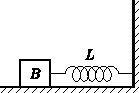
\includegraphics{figure/fig03.02b}
    }
    \hfill
    \subfigure[]{
        \label{fig:03.02c}
        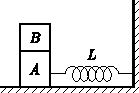
\includegraphics{figure/fig03.02c}
    }
    \hfill
    \label{fig:03.02}
    \caption{牛顿第二定律的含义}
\end{figurex}
% 093.jpg
\clearpage
\noindent 们做三个实验。其一,物体$ A $与一弹簧相连,把弹簧拉长到$ L $,然后
释放物体$ A $,在弹簧的牵动下,$ A $作加速运动,测量出开始时刻的
加速度$ a_A $;其二,用上述弹簧与物体$ B $相连,仍拉长到$ L $,测出
释放时刻的加速度$  a _ { B  } $;  其三,仍是上述弹簧,拉长到$ L $,和捆在
一起的$ A $,$ B $相连,测出释放时刻的加速度$  a _ { A B }  $。

上述三个实验,只用了运动学的概念,测得了一组数据,如
果没有其他知识,我们就不能得到更多的东西。现在,我们看如
何用动力学来得到的测量量$ a_A $,$ a_B $,$ a_{AB} $之间的联系。

我们可以取物体$ A $的质量作为质量单位的标准,故可任意定
其数值为$ m_A $,利用式\eqref{eqn:03.02.01}作为力的定义,再由实验\subref{fig:03.02a}测得
的$ a $即可算出弹簧对$ A $的牵动力
\begin{equation}\label{eqn:03.02.02}
    F = m _ { A } a _ { A }
\end{equation}

在实验\subref{fig:03.02b}中,设弹簧对$ B $的牵动力与牵动$ A $时一样,仍为$ F $,
则利用式\eqref{eqn:03.02.01}作为质量的定义,可算出$ B $的质量
\begin{equation}\label{eqn:03.02.03}
    m _ { B } = \frac { F } { a _ { B } }
\end{equation}

在实验\subref{fig:03.02a}中,如果假设$ A $与$ B $在一起的质量$ m_{AB} $是分别质量
之和(即质量是可加的):
\begin{equation}\label{eqn:03.02.04}
    m _ { A B } = m _ { A } + m _ { B }
\end{equation}

再假定牵动力依然是F,就可以用式\eqref{eqn:03.02.01}作为定律,来预
言此时的加速度$ a_{AB} $为
\begin{equation}\label{eqn:03.02.05}
    a _ { A B } = \frac { F } { m _ { A B } } = \frac { F } { m _ { A } + m _ { B } } = \frac { a _ { A } a _ { B } } { a _ { B } + a _ { A } }
\end{equation}

{\ziju{-0.005}我们注意到,式\eqref{eqn:03.02.05}中只含有实验直接可测的量(与我们
任意取定$ m_A $值无关),亦即牛顿第二定律给出了从一组实验〔\subref{fig:03.02a},\subref{fig:03.02b}〕的数据计算另一实验〔\subref{fig:03.02c}〕的规则。如果这样计算出来的结果
与观测值符合,就为牛顿第二定律的正确性提供了一个实验验证。
这样一个理论与实验之间的全面关系告诉我们什么呢?}

% 094.jpg
(1) 在整个分析过程中,我们的确有时将式\eqref{eqn:03.02.01}作为定义
使用,有时又作为定律,但在每个具体环节上它的作用都是明确
的,并没有同时既作定义,又作定律的情况,因而是不“混乱”
的。理论与实验之间由一些测量操作联系着,由此就不难理解式
\eqref{eqn:03.02.01}既是定义又是定律、“身兼两任”的实质。

(2) 式\eqref{eqn:03.02.05}中都是实验可以直接测定的量,也就是说,由
式\eqref{eqn:03.02.01}所给出的预言是明确的,具有可验证性或可否证性。

(3) 物理学的规律,例如牛顿第二定律,都有一定的适用限
度。在限度之外,牛顿第二定律不再成立。在牛顿第二定律不适
用的范围,用它来预言实验就不再正确,因而这时用它来作为定
义也就没有意义了。或者说,当式\erratanote{\eqref{eqn:03.02.01}}{原书作“3.3.1”,显误。}作为定律不再适用时,
用它作为力及质量的定义就也不适用了。上述力及质量的定义也
有其适用限度。这种“定义”显然与数学中所用定义的含义有很
大差别。

(4) 只依靠牛顿第二定律来分析运动性质,还是不够的,必须
扩充其他假定,才有可能预测运动。在上例中,不仅用了式\eqref{eqn:03.02.01},
而且用了两个假定:弹簧被拉长到同样的长度时产生同样
的牵动力F;质量具有可加性。这个特点也与数学不相同。数学
上的已知到求证之间,只能使用定理、定义进行逻辑推理,不外
加其他东西。但物理上没有一个是如此。必定要补充一些外加的
假设,才能从已知测量中作出预言。外加的假设,反映了我们对
客观世界的看法,或者说是客观世界的一种模型。在什么地方应
当补充些什么,或者说用什么模型去看客观世界,这是物理的难
点,而这也正是物理学工作的精髓。

{\ziju{-0.01} 这样,我们就说明了牛顿第二定律既是动力学基本规律,同
时又可作为质量及力的定义的全部意义。当然,这并不排斥我们
去寻求不依赖于牛顿第二定律的关于质量及力的定义。但是,即
使我们找到了更深入的定义,那么在牛顿第二定律适用的范围内,
% 095.jpg
新的定义也必定等价于本节所述的定义。因此,在牛顿第二定律
适用的范围中,采用上述定义不仅是正确的,而且是“够用”的
了。}

按式\eqref{eqn:03.02.01},力是一个矢量,它的合成、分解遵守矢量代数
运算法则。质量是一个标量。

式\eqref{eqn:03.02.01}是一个矢量方程,它等价于三个分量方程:
\begin{equation*}
    F = m a _ { x } \quad F _ { y } = m a _ {y} \quad F _ { z } = m a_ { z }
\end{equation*}

质量的单位是千克,千克的标准是保存在国际计量局中的一
个铂铱圆柱体。在原子尺度上,利用原子质量单位,用$^{12}$C作它
的标准,国际协议规定$^{12}$C的原子质量精确地等于12个原子质量
单位。原子质量单位与千克的关系是:
\begin{equation*}
    1\text{原子质量单位} = \num{1.6605655e-27}\text{千克}
\end{equation*}

力的单位是牛顿,一牛顿力使质量为一千克的物体产生$1\text{米/秒}^2$
的加速度。